%----------------------------------------------------------------------------------------
%	PACKAGES AND OTHER DOCUMENT CONFIGURATIONS
%----------------------------------------------------------------------------------------

\documentclass[paper=a4, fontsize=11pt]{scrartcl} % A4 paper and 11pt font size

\usepackage[T1]{fontenc} % Use 8-bit encoding that has 256 glyphs
\usepackage{fourier} % Use the Adobe Utopia font for the document - comment this line to return to the LaTeX default
\usepackage[english]{babel} % English language/hyphenation
\usepackage{amsmath,amsfonts,amsthm, amssymb} % Math packages
\usepackage[utf8]{inputenc}

\usepackage{graphicx}
\usepackage{float}

\usepackage{lipsum} % Used for inserting dummy 'Lorem ipsum' text into the template

\usepackage{sectsty} % Allows customizing section commands
\allsectionsfont{\centering \normalfont\scshape} % Make all sections centered, the default font and small caps

\usepackage{fancyhdr} % Custom headers and footers
\pagestyle{fancyplain} % Makes all pages in the document conform to the custom headers and footers
\fancyhead{} % No page header - if you want one, create it in the same way as the footers below
\fancyfoot[L]{} % Empty left footer
\fancyfoot[C]{} % Empty center footer
\fancyfoot[R]{\thepage} % Page numbering for right footer
\renewcommand{\headrulewidth}{0pt} % Remove header underlines
\renewcommand{\footrulewidth}{0pt} % Remove footer underlines
\setlength{\headheight}{13.6pt} % Customize the height of the header

\numberwithin{equation}{section} % Number equations within sections (i.e. 1.1, 1.2, 2.1, 2.2 instead of 1, 2, 3, 4)
\numberwithin{figure}{section} % Number figures within sections (i.e. 1.1, 1.2, 2.1, 2.2 instead of 1, 2, 3, 4)
\numberwithin{table}{section} % Number tables within sections (i.e. 1.1, 1.2, 2.1, 2.2 instead of 1, 2, 3, 4)

\setlength\parindent{0pt} % Removes all indentation from paragraphs - comment this line for an assignment with lots of text

%----------------------------------------------------------------------------------------
%	TITLE SECTION
%----------------------------------------------------------------------------------------

\newcommand{\horrule}[1]{\rule{\linewidth}{#1}} % Create horizontal rule command with 1 argument of height

\title{	
    \normalfont \normalsize 
    \textsc{TDT4173 - Machine Learning \& Case-based Reasoning, IDI, NTNU} \\ [25pt] % Your university, school and/or department name(s)
    \horrule{0.5pt} \\[0.4cm] % Thin top horizontal rule
    \huge Assignment 5 \\ % The assignment title
    \horrule{2pt} \\[0.5cm] % Thick bottom horizontal rule
}

\author{Peter Aaser, Mathias Ose \& Øyvind Robertsen} % Your name

\date{\normalsize\today} % Today's date or a custom date

\begin{document}

\maketitle % Print the title

\section{System Overview}
The system is implemented in Python 3, using the libraries \texttt{scikit-learn}, \texttt{scikit-images}, \texttt{Pillow}, \texttt{numpy}, \texttt{matplotlib}.

The system is written in a modular fashion, allowing us to easily swap in and out preprocessing functions or classifier models.
The libraries used do most of the heavy lifting, with our task as programmers mostly just to compose the library functions in a sensible way.

\hspace{0.25cm}

A typical use-case is something like:
    \begin{enumerate}
        \item   Select a classifier model, preprocessing function and various other parameters.
        \item   Load dataset and split into training set and test set.
        \item   Preprocess the training set and train the selected classifier on it.
        \item   Preprocess the test set and have the trained classifier classify the set.
        \item   Assess the success rate of the classifier test.
        \item   Load a test image and use the sliding windows function to extract samples from it.
        \item   Have the trained learner classify these samples.
        \item   Output the results on top of the image.
    \end{enumerate}

Various experiments have been stored as `.py` files that can be run from command line.

\section{Preprocessing}

We tested several preprocessing techniques and combinations thereof,
such as morphological closing, binarisation and histogram of gradients
analysis.  A combination of binarization and histogram of gradients
analysis yielded the best results in combination with the classifier
we chose.

All attempts at including morphology-based techniques to reduce noise,
degraded performance.  While for instance erosion might reduce
unwanted noise in images, it is not very discriminatory about what it
removes, resulting in key features being removed from images.

Histogram of gradients analysis partitions the image into cells and
outputs a vector of gradients, one for each cell.  Inspired by He et
al~\cite{bib:spp}, we perform several rounds of analysis, with varying
cell dimensions, and combine the results, to better correlate features
spatially in the feature vectors. This also makes our classifier
resolution independent.

Figure~\ref{fig:preprocessing} illustrates our preprocessing pipeline.

\begin{figure}[H]
    \centering
    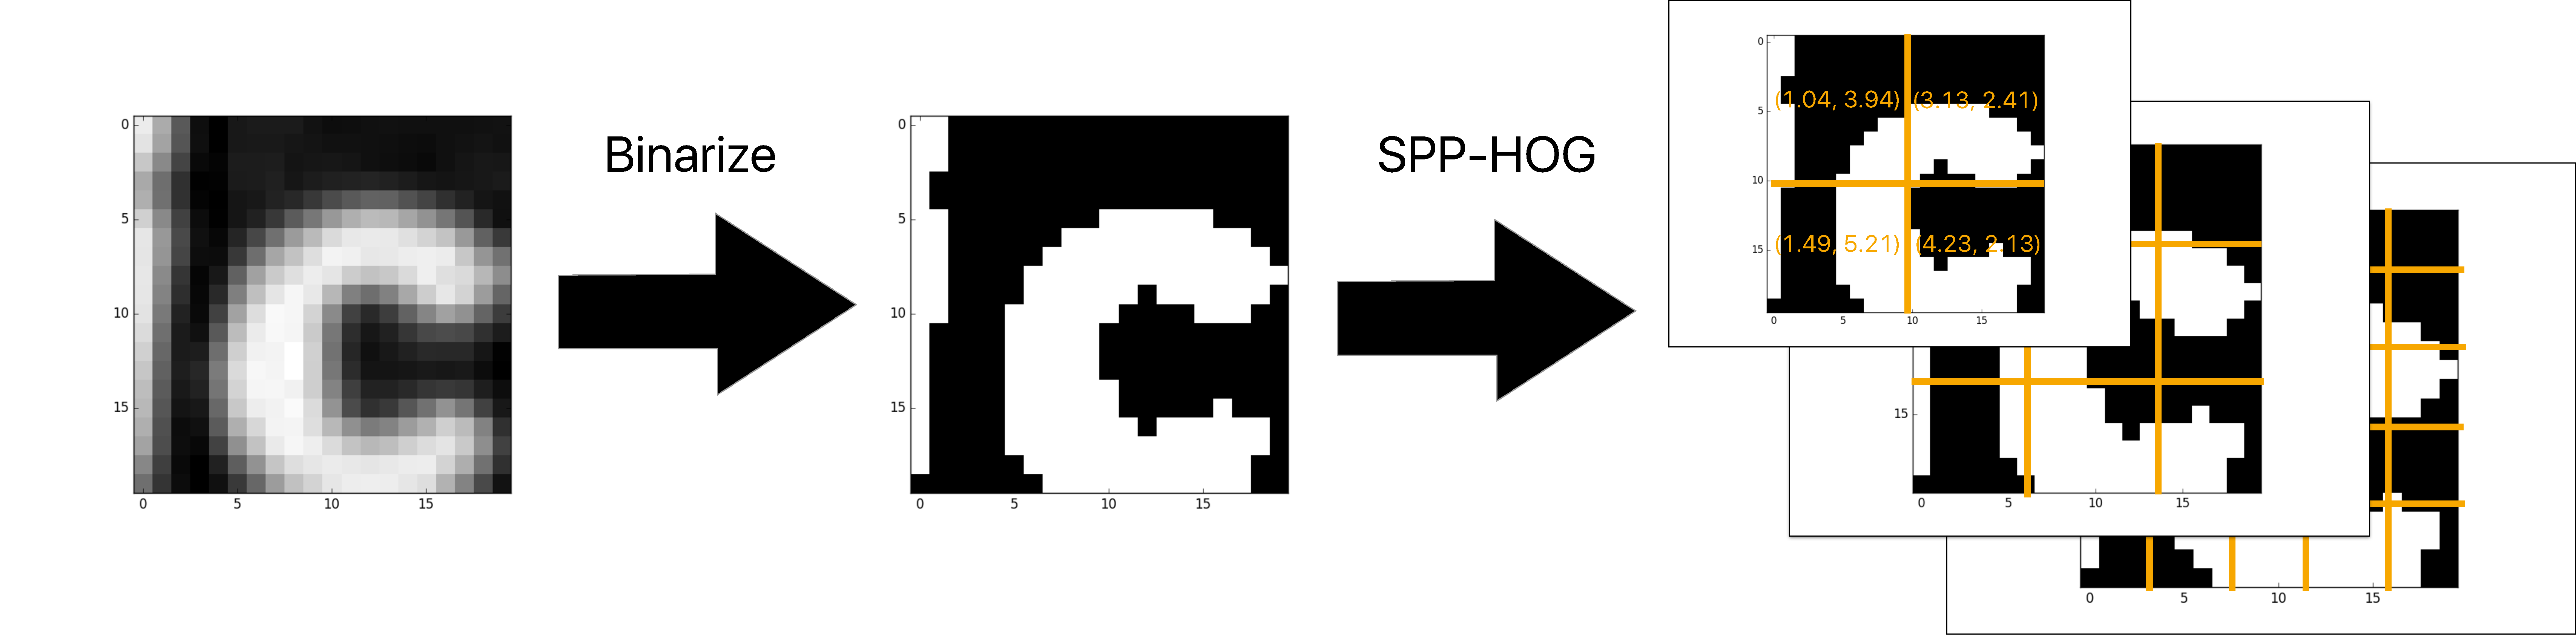
\includegraphics[width=0.8\linewidth]{img/preprocessing.pdf}
    \caption{Preprocessing steps} \label{fig:preprocessing}
\end{figure}

\section{Classifiers}
\subsection{SVC}
Our approach to classifiers was driven by our lack of experience with
using machine learning frameworks.  When starting out we used a
tutorial for recognizing hand written digits provided by scikit which
happened to use a support vector classifier.\\
In our first attempt we simply extended the example from sklearn to
create a dataset from 74k-lite to see what kind of performance we
would get.  After getting very lackluster results we first thought
there was an error in our program, a test run using only the a's and
b's predicted only a's which made us spend time debugging.  A quick
look on the datasets revealed why we were wrong: the example we
followed used a set of 10*10 images which were all cleanly written.\\
Compared to our pictures which featured many different fonts and four
times as many pixels the task of classifying the example images was
much smaller.  Realizing this we tried implementing some preprocessors
to see how our classifiers fared with inputs featuring lower
dimensionality.  Returning to the classifier we resumed our trials
with our arbitrarily chosen SVC.\\  The standard sklearn SVC
implementation uses an rbf kernel, standing for radial basis function
network.  Because we did not know how rbf worked we decided to try out
a linear kernel instead.  This made sense not only because of the
approachability compared to the complex rbf implementation, but also
because we had a somewhat intuitive understanding of why it could
perform well.\\  With our radial orientation scheme we predicted that
the amount of angled surfaces in letters would be linearly separable
allowing the linear SVC to perform well.  We can't be sure whether
this intuition was correct, but we got very nice results, handily
beating our initial rbf kernel implementation.\\  One flaw with using an
svm is that our dataset consists of both small and big letters,
essentially creating "islands" which would make it hard to partition
the feature space into partitions consisting both of the big and small
version of a letter.  We are unsure how the SVM in scikit is
implemented, it is possible that several clusters may be formed for
the same class which would explain why it performed so well, or
perhaps the SVC found a way to create partitions containing both the
small and the big version for each letter.\\  The best result we
obtained with a linear classifier was a precision of 0.78 which was
achieved when first binarizing the images and then applying HOG.\\
We expected HOG to perform fairly well on images without
applying binarization as HOG should be able to deal with noise.  With
no binarization the classifier reached a score of 0.76 which tells us
that while HOG pulls most of the weight the additional step of
binarization is still worthwhile, yielding an ~8\% reductiong of
missclassifications.  The following table shows the performance of our
SVC using different parameters:
\begin{table}[H]
    \centering
    \begin{tabular}{l | l | l}
        Kernel & preprocessing & precision\\ \hline
        Linear & binarization \& HOG & 0.78 \\ \hline
        Linear & binarization & 0.11 \\ \hline
        Linear & HOG & 0.76\\ \hline
        RBF & binarization \& HOG & 0.76\\
    \end{tabular}
    \caption{Performance for different configurations using SVC}
\end{table}

\subsection{K Nearest neighbors}
In order to test out our theory that an SVC would suffer from
different versions of letters we settled on k nearest neighbors as a
second classifier.  We hypothesized that this method would perform
better based on our suspected weakness of the SVC since nearest
neighbours does not rely on partitioning the feature space.  Our best
performing configuration managed a precision of 0.81 using 10
neighbours linearly weighted by manhattan distance, yielding a fairly
decent improvement.  Not only did K nearest outperform SVC, it also
did so without having to use the binarization preprocessing step.
We're not sure why binarization is nescessary using SVC compared to K
nearest % postuler no greier her..? % The following table shows the
performance of our K nearest classifier using different parameters:

\begin{table}[H]
    \centering
    \begin{tabular}{l | l | l | l | l}
        K (neighbors) & weight & distance measure & preprossesing & precision\\ \hline
        10 & linear distance & euclidean & HOG & 0.80\\ \hline
        10 & uniform & euclidean & HOG & 0.79\\ \hline
        5 & uniform & euclidean & HOG & 0.79\\ \hline
        10 & linear & manhattan & HOG & 0.81\\ \hline
        10 & linear & manhattan & HOG \& binarization & 0.81\\
    \end{tabular}
    \caption{Performance for different configurations using a K nearest neighbors classifier}
\end{table}

\section{Detection}
The sliding windows algorithm has been implemented as described in the project
description.
The samples from this algorithm can be assessed by the trained classifier,
as long as the number of features in each processed window is the same as the classifier was trained on.

To test the detection we took a photo of a sheet of paper with some text and drawings.
The sheet has text of two different sizes, as well as some drawings of non-text.
The edges of the sheet, as well as of the table the sheet lies upon.
The window size of the sliding window algorithm is fitted to the larger text.
Running the classifier on the windows, we can visualise the results by selecting the windows where the confidence of the classifier is above a specific threshold, and draw an indicator on top of the photo.
An example of this can be seen in Figure \ref{fig:illuminati}.
As we can see, the detector does higlight where there is text to some degree,
but it is also tripped up by the drawings and somee edges in the "background".

\begin{figure}[H]
    \centering
    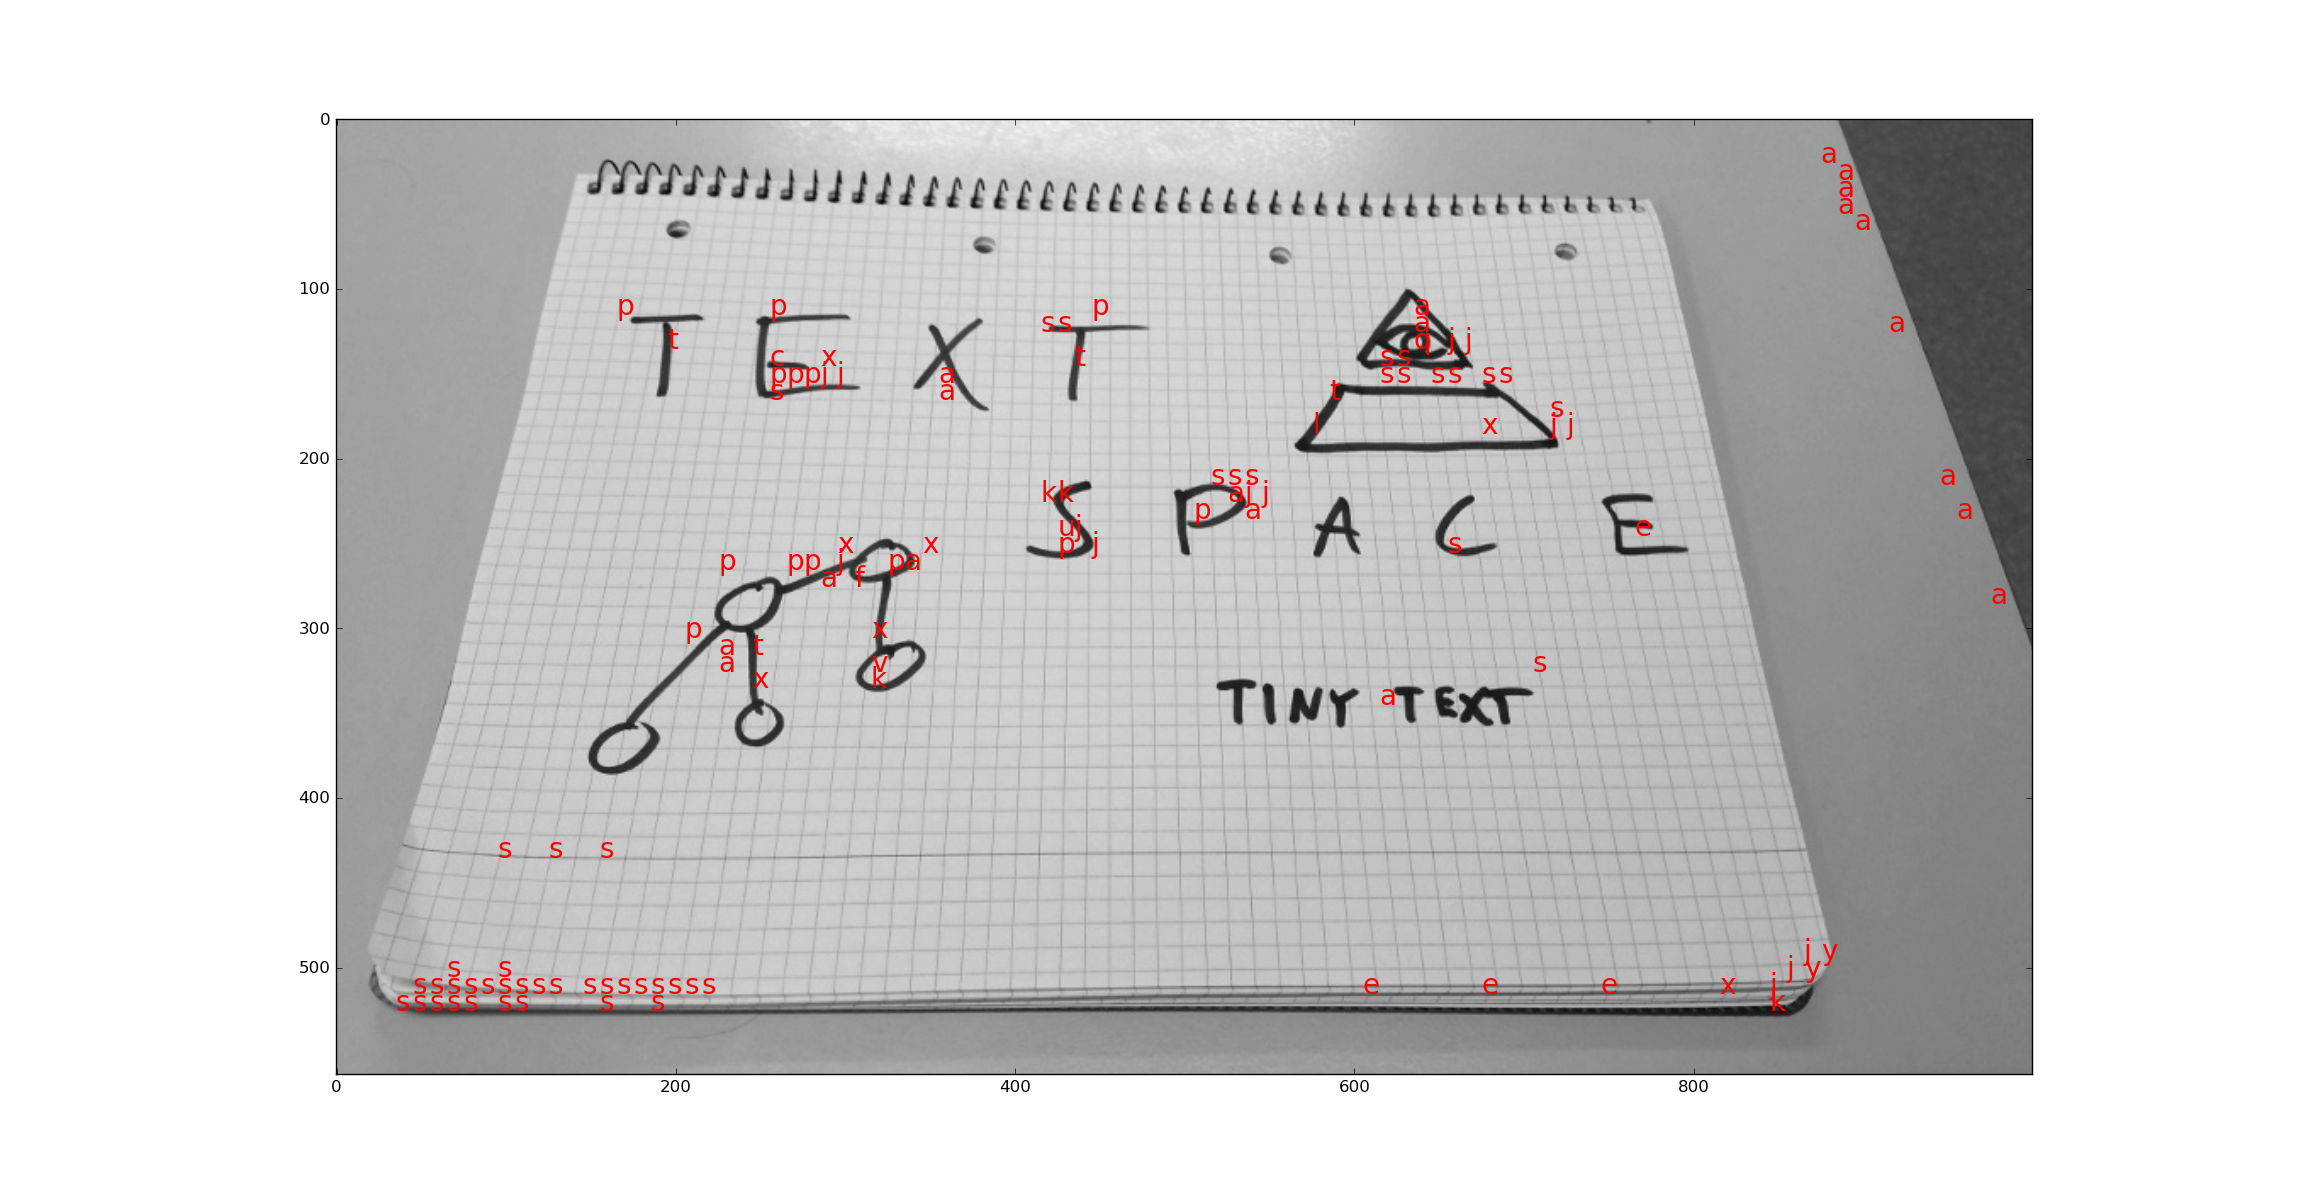
\includegraphics[width=\linewidth]{img/illuminati}
    \caption{Detection results.}
    \label{fig:illuminati}
\end{figure}

We tried different methods and parameters for this experiment.
The best results are seen in Figure \ref{fig:illuminati},
with the relevant parameters shown in Table \ref{tbl:illuminati}.

\begin{table}[H]
    \centering
    \begin{tabular}{l|l}
        Preprocessing   &   \texttt{oriented\_gradients}    \\\hline
        Classifier      &   \texttt{LinearSVC}              \\\hline
        Threshold       &   $0.5$
    \end{tabular}
    \caption{Parameters for experiment seen in Figure \ref{fig:illuminati}}.
    \label{tbl:illuminati}
\end{table}

This experiment has been stored to the file \texttt{experiment\_detection\_photo\_hog\_svc.py} and can be recreated by running it.

An interesting observation at this stage is how adding the binarization preprocessing before the HOG preprocessing changes the outcome.
This increases the number of false positives drastically around the edges of the paper in the photo.
The binarization is accentuating the edges and this creating something which looks like letters to the classifier.
Looking closer at what letters the classifier thinks it is seeing near the edges, we see things like "i" and "l", which supports this assumption.



\subsection{Evaluation}
Considering our lack of experience with text recognition we are fairly happy with how well the classifier performs.
If we had more time we would like to try more advanced techniques such as convolutional neural nets to see if they could do any better.
Another interesting idea is combinining both the SVC and the K nearest neighbors classifiers as an ensemble to study how the performance would improve, 
investigating how dominant the k nearest neighbors classifier really is.

We feel that the strongest component of our system is the spatial-pyramid-pooling inspired HOG analysis.
It very effectively reduces dimentionality of the feature vector, while still expressing how shapes in the image correlate spatialy.
It is also makes the system resolution independent, making it easier to use for our detector.

On the other hand, we feel the detector is the weakest part.
It performs reasonable when there is little going on in the image.
Images with complex handwriting and many other features apart from letters, will cause it to yield false positives.
Arguably, this is also a fault with our preprocessor, as one way of improving this performance would be to intelligently remove noice in that step.


\bibliographystyle{plain}
\bibliography{references.bib} 

\end{document}
